\documentclass[11pt]{article}
\usepackage{amssymb}
\usepackage{amsthm}
\usepackage{enumitem}
\usepackage{amsmath, physics}
\usepackage{bm}
\usepackage{adjustbox}
\usepackage{mathrsfs}
\usepackage{graphicx}
\usepackage{siunitx}
\usepackage[mathscr]{euscript}

\title{\textbf{Solved selected problems of Modern Physics for Scientists and Engineers - John Taylor}}
\author{Franco Zacco}
\date{}

\addtolength{\topmargin}{-3cm}
\addtolength{\textheight}{3cm}

\newcommand{\N}{\mathbb{N}}
\newcommand{\Z}{\mathbb{Z}}
\newcommand{\Q}{\mathbb{Q}}
\newcommand{\R}{\mathbb{R}}
\newcommand{\diam}{\text{diam}}
\newcommand{\cl}{\text{cl}}
\newcommand{\bdry}{\text{bdry}}
\newcommand{\inter}{\text{int}}
\newcommand{\hatx}{\bm{\hat{x}}}
\newcommand{\haty}{\bm{\hat{y}}}
\newcommand{\hatz}{\bm{\hat{z}}}
\newcommand{\hatrho}{\bm{\hat{\rho}}}
\newcommand{\hatphi}{\bm{\hat{\phi}}}
\newcommand{\hatr}{\bm{\hat{r}}}
\newcommand{\hattheta}{\bm{\hat{\theta}}}

\theoremstyle{definition}
\newtheorem*{solution*}{Solution}
\renewcommand*{\proofname}{\bf{Solution}}

\begin{document}
\maketitle
\thispagestyle{empty}

\section*{Chapter 3 - Atoms}

\begin{proof}{\textbf{3.3}}
    We know that the ratio of the masses of the $H_2O$ atoms is
    $$\frac{m_O}{2m_H} = \frac{15.999}{2\times 1.008}$$
    so we need a mass of $2~g \times 15.999/2.016  = 15.872~g$ of oxygen to
    form water with $2~g$ of hydrogen.
\end{proof}
\begin{proof}{\textbf{3.6}}
\begin{itemize}
    \item [\textbf{(a)}] To form carbon monoxide $CO$ with $1~g$ of carbon
    we need 
    $$1~g \times \frac{15.999}{12.011} = 1.332~g$$
    of oxygen given that the atomic mass of carbon is $12.011$.

    \item [\textbf{(b)}] To form carbon dioxide $CO_2$ with $1~g$ of carbon
    we need
    $$1~g \times \frac{2 \times 15.999}{12.011} = 2.664~g$$
    of oxygen, where in this case we have 2 masses of oxygen to account for.
\end{itemize}
\end{proof}
\cleardoublepage
\begin{proof}{\textbf{3.7}}
    \begin{center}
        \begin{tabular}{|l|l|l|l|l|} \hline
                  & He & Li & Na & Ca \\ \hline
        electrons & 2  & 3  & 11 & 20 \\ \hline
        protons   & 2  & 3  & 11 & 20 \\ \hline
        neutrons  & 2  & 4  & 12 & 20 \\ \hline
        nucleons  & 4  & 7  & 23 & 40 \\ \hline
    \end{tabular}
    \end{center}
\end{proof}
\begin{proof}{\textbf{3.16}}
Correct to the nearest $u$ these are the masses of the listed molecules
\begin{itemize}
    \item [(a)] $H_2O$:
    $$(1.008~u \times 2) + 15.999~u =  18.015~u \approx 18~u$$
    \item [(b)] $N_2O$:
    $$(14.007~u \times 2) + 15.999~u =  44.013~u \approx 44~u$$
    \item [(c)]
    $O_3$: 
    $$15.999~u \times 3 = 47.997~u \approx 48~u$$
    \item [(d)] $C_6H_{12}O_6$:
    \begin{align*}
        (12.011~u \times 6) + (1.008~u \times 12) + (15.999~u \times 6)
        &= 180.156~u \\
        &\approx 180~u
    \end{align*}
    \item [(e)] $NH_{3}$:
    $$14.007~u + (1.008~u \times 3) =  17.031~u \approx 17~u$$
    \item [(d)] $CaCO_{3}$:
    $$40.078~u + 12.011~u + (15.999~u \times 3) =  100.086~u \approx 100~u$$
\end{itemize}
\end{proof}
\begin{proof}{\textbf{3.17}}
\begin{itemize}
    \item [(a)]
    \begin{itemize}
        \item Ne $: Z = 10$ $\rightarrow$ ratio: $20.180 / 10 = 2.018$
        \item Ca $: Z = 20$ $\rightarrow$ ratio: $40.078 / 20 = 2.004$
        \item Zn $: Z = 30$ $\rightarrow$ ratio: $65.380 / 30 = 2.179$
        \item Zr $: Z = 40$ $\rightarrow$ ratio: $91.224 / 40 = 2.281$
        \item Sn $: Z = 50$ $\rightarrow$ ratio: $118.711 / 50 = 2.374$
        \item Nd $: Z = 60$ $\rightarrow$ ratio: $144.243 / 60 = 2.404$
        \item Yb $: Z = 70$ $\rightarrow$ ratio: $173.055 / 70 = 2.472$
        \item Hg $: Z = 80$ $\rightarrow$ ratio: $200.59 / 80 = 2.507$
        \item Th $: Z = 90$ $\rightarrow$ ratio: $232.038 / 90 = 2.578$
    \end{itemize}
    \item [(b)] If $A$ is close to $2Z$ then given that $A = Z + N$ we get that
    $2Z \approx Z + N$ and therefore this implies that $N \approx Z$.
\end{itemize}
\end{proof}
\begin{proof}{\textbf{3.24}}
    \begin{itemize}
        \item [(a)] A mole of $CO_2$ weights about
        $44~\text{grams}$ so $1~\text{gram}$ of $CO_2$ will contain
        the following amount of $C$ atoms
        \begin{align*}
            1&~\text{gram} \times \frac{1~\text{mol}}{44~\text{gram}}
            \times \frac{6.022\times 10^{23}~CO_2\text{ molecules}}{1~\text{mol}}
            \times \frac{1~\text{C atom}}{1~CO_2\text{ molecule}} =\\
            &= 1.368\times 10^{22}~\text{C atoms}
        \end{align*}
        In the same way, there are 
        \begin{align*}
            1&~\text{gram} \times \frac{1~\text{mol}}{44~\text{gram}}
            \times \frac{6.022\times 10^{23}~CO_2\text{ molecules}}{1~\text{mol}}
            \times \frac{2~\text{O atom}}{1~CO_2\text{ molecule}} =\\
            &= 2.737\times 10^{22}~\text{O atoms}
        \end{align*}
        Therefore the fraction of $C$ atoms is
        \begin{align*}
            \frac
            {1.368\times 10^{22}~\text{C atoms}}
            {
                1.368\times 10^{22}~\text{C atoms}
                + 2.737\times 10^{22}~\text{O atoms}
            }
            = 0.333 
        \end{align*}
        Finally, the mass of $C$ atoms in 1 gram of $CO_2$ is
        \begin{align*}
            1.368\times 10^{22}~\text{C atoms}
            \times \frac{12~\text{grams}}{6.022\times 10^{23}~\text{C atoms}}
            &= 0.272~\text{grams}
        \end{align*}
        Which implies that the fraction of mass in $C$ is
        \begin{align*}
            \frac{0.272~\text{C grams}}{1~CO_2\text{ grams}} = 0.272
        \end{align*}

        \item [(b)] A mole of $CH_4$ contains
        $6.022\times 10^{23}~CH_4\text{ molecules}$ then
        \begin{align*}
            6.022\times 10^{23}~CH_4\text{ molecules}
            \times \frac{1~\text{C atom}}{1~CH_4\text{ molecule}}
            = 6.022\times 10^{23}~\text{C atoms}
        \end{align*}
        In the same way, there are 
        \begin{align*}
            6.022\times 10^{23}~CH_4\text{ molecules}
            \times \frac{4~\text{H atoms}}{1~CH_4\text{ molecule}}
            = 2.408\times 10^{24}~\text{H atoms}
        \end{align*}
        Therefore the fraction of $C$ atoms is
        \begin{align*}
            \frac
            {6.022\times 10^{23}~\text{C atoms}}
            {
                6.022\times 10^{23}~\text{C atoms}
                + 2.408\times 10^{24}~\text{H atoms}
            }
            = 0.2
        \end{align*}
        Finally, the mass of $C$ atoms in 1 mol of $CH_4$ is
        \begin{align*}
            6.022\times 10^{23}~\text{C atoms}
            \times \frac{12~\text{grams}}{6.022\times 10^{23}~\text{C atoms}}
            &= 12~\text{grams}
        \end{align*}
        Which implies that the fraction of mass in $C$ is
        \begin{align*}
            \frac{12~\text{C grams}}{16~CH_4\text{ grams}} = 0.75
        \end{align*}

        \item [(c)] A mole of $C_2H_6$ contains
        $6.022\times 10^{23}~C_2H_6\text{ molecules}$ then we have that
        \begin{align*}
            1000&~C_2H_6\text{ mol}
            \times
            \frac{6.022\times 10^{23}~C_2H_6\text{ molecules}}{1~C_2H_6\text{ mol}}
            \times \frac{2~\text{C atom}}{1~C_2H_6\text{ molecule}}\\
            &= 1.204\times 10^{27}~\text{C atoms}
        \end{align*}
        In the same way, there are 
        \begin{align*}
            1000&~C_2H_6\text{ mol}
            \times
            \frac{6.022\times 10^{23}~C_2H_6\text{ molecules}}{1~C_2H_6\text{ mol}}
            \times \frac{6~\text{H atoms}}{1~C_2H_6\text{ molecule}}\\
            &= 3.613\times 10^{27}~\text{H atoms}
        \end{align*}
        Therefore the fraction of $C$ atoms is
        \begin{align*}
            \frac
            {1.204\times 10^{27}~\text{C atoms}}
            {
                1.204\times 10^{27}~\text{C atoms}
                + 3.613\times 10^{27}~\text{H atoms}
            }
            = 0.249
        \end{align*}
        Finally, the mass of $C$ atoms in 1000 moles of $C_2H_6$ is
        \begin{align*}
            1.204\times 10^{27}~\text{C atoms}
            \times \frac{12~\text{grams}}{6.022\times 10^{23}~\text{C atoms}}
            &= 23992.03~\text{grams}
        \end{align*}
        Which implies that the fraction of mass in $C$ is
        \begin{align*}
            \frac{23992.03~\text{C grams}}{(1000 \times 30)~C_2H_6\text{ grams}}
            = 0.799
        \end{align*}

    \end{itemize}    
\end{proof}
\begin{proof}{\textbf{3.25}}
    From the ideal gas law, we know that $pV = N k_B T$ where $N$ is the number
    of molecules and $k_B$ is Boltzmann's constant. Hence we see that
    $N/V = p/k_B T$ where $N/V$ is the number of molecules per volume
    or the number density of molecules.
\end{proof}
\cleardoublepage
\begin{proof}{\textbf{3.27}}
    By multiplying the ideal gas law by the molar mass $M_{He}$ of $He$
    we get that
    \begin{align*}
        M_{He}(pV) &= M_{He}(n R T)\\
        \frac{pM_{He}}{RT} &= \frac{m_{He}}{V}\\
        \rho_{He} &= \frac{pM_{He}}{RT}
    \end{align*}
    Where we used that $M_{He}n = m_{He}$ which is the mass of $He$
    also, we used that $m_{He}/V = \rho_{He}$ is the density of $He$.
    Therefore by replacing the $\rho_{He}$ by $\rho_{H_2O}$ and the values of
    $M_{He} = 4~g/mol$ and $T = 300~K$ we get that $p$ is
    \begin{align*}
        p &= \frac{\rho_{H_2O}RT}{M_{He}}\\
        &= \frac{ 997048 ~g/m^3 \cdot 8.314~J/K mol \cdot 300~K}{4~g/mol}\\
        &= 621709280.4~\frac{J}{m^3} \cdot \frac{1~atm}{1.01 \times 10^5~N/m^2}\\
        &= 6155.53~atm
    \end{align*}
\end{proof}
\cleardoublepage
\begin{proof}{\textbf{3.30}}
    Let us consider a container of oxygen gas at $T = 237~K$ and
    $p = 1~atm = 1.01\times 10^5~N/m^2$
    \begin{itemize}
        \item [(a)] First, we need to determine the $O_2$ molecule mass in kg
        \begin{align*}
            m = \frac{32~g/mol}{6 \times 10^{23}~molecules/mol}
            = 5.33 \times 10^{-23} ~kg/molecule
        \end{align*}
        The collision cross-section in this case is given by
        \begin{align*}
            \sigma = \pi(2R)^2 = 4\pi(0.15 \times 10^{-9}~m)^2
            = 2.8 \times 10^{-19}~m^2
        \end{align*}
        and the number density is
        \begin{align*}
            n = \frac{N}{V} = \frac{p}{kT}
            = \frac{1.01\times 10^5~N/m^2}{(1.38 \times 10^{-23}~J/K)(237~K)}
            = 3.088 \times 10^{25}~m^{-3}
        \end{align*}
        Finally, by solving equation (3.34) for time $t$ we get that
        \begin{align*}
            t &= (D_{rms})^2n\sigma\sqrt{\frac{m}{3kT}}\\
            &=1^2 \cdot (3.088 \times 10^{25})
            \cdot (2.8 \times 10^{-19})
            \cdot \sqrt{\frac{5.33 \times 10^{-23}}{
                3\cdot(1.38 \times 10^{-23})\cdot(237)}}\\
            &= 637271.628~s \approx 7~days
        \end{align*}
        \item [(b)] At a pressure of $0.01~atm$ we have a number density of
        \begin{align*}
            n = \frac{N}{V} = \frac{p}{kT}
            = \frac{1013.25~N/m^2}{(1.38 \times 10^{-23}~J/K)(237~K)}
            = 3.098 \times 10^{23}~m^{-3}
        \end{align*}
        Hence it would take the molecule the following time to reach $1~m$
        distance from its starting point.
        \begin{align*}
            t &= (D_{rms})^2n\sigma\sqrt{\frac{m}{3kT}}\\
            &=1^2 \cdot (3.098 \times 10^{23})
            \cdot (2.8 \times 10^{-19})
            \cdot \sqrt{\frac{5.33 \times 10^{-23}}{
                3\cdot(1.38 \times 10^{-23})\cdot(237)}}\\
            &= 6393.35~s = 1.77~hours
        \end{align*}
        \item [(c)] knowing that $n = p/kT$ and $D_{rms} = \sqrt{N} d$ then
        by replacing these values in the equation we have for time $t$
        we get that
        \begin{align*}
            Nd^2\frac{p\sigma}{kT}\sqrt{\frac{m}{3kT}} &= t\\
            Nd^2\frac{p\sigma}{kT} &= t\sqrt{\frac{3kT}{m}}\\
            p &= \frac{tkT}{Nd^2\sigma}\sqrt{\frac{3kT}{m}}\\
        \end{align*}

    \end{itemize}
\end{proof}
\cleardoublepage
\begin{proof}{\textbf{3.36}}
    Let us consider a cubical container filled with  a gas of molecules with
    number density $n$.
    Let us consider two sets of molecules, one set of molecules
    is traveling to the right (in the positive $x$-direction)
    and the other set to the left (in the negative $x$-direction)
    both with the same velocity $|v_x|$.
    Let us consider in particular the molecules which are at a distance
    $\Delta x$ from the wall where $\Delta x \ll \lambda$ where $\lambda$
    is the mean free path. In this situation, the molecules will not collide
    with any other molecules before hitting the wall, hence given that
    every molecule is moving with the same velocity the change
    in momentum will be
    $\Delta p_{x} = p_x^{final} - p_x^{initial} = -2mv_{x}$ so the average
    force applied to the wall by one molecule is the change in momentum between
    collisions divided by the average time $\Delta t$ thus
    \begin{align*}
        F_{x} = \frac{N}{2}\frac{|\Delta p_{x}|}{\Delta t}
        = \frac{N}{2}\frac{2m|v_{x}|}{\Delta x/|v_{x}|}
        = N\frac{mv_{x}^2}{\Delta x}
    \end{align*}
    Where we multiplied by the number of molecules $N/2$ to account for every
    molecule hitting the wall in this direction, the other half $N$ hits
    the opposite wall.
    The average pressure on the wall is then obtained as follows
    \begin{align*}
        p = \frac{F_x}{A}
        = \frac{Nm v_x^2}{A\Delta x}
        = nm v_x^2
    \end{align*}
    Where we used that $n = N/(A\Delta x)$ is the number density.
    Also, if we compute in the same way the pressure for the rest of the walls
    where we take $\Delta y = \Delta z = \Delta x$ and $v_x^2 = v_y^2 = v_z^2$
    we get that
    \begin{align*}
        p &= 2\frac{F_x}{A} + 2\frac{F_y}{A} + 2\frac{F_z}{A}\\
        &= \frac{2Nm v_x^2}{A \Delta x} + \frac{2Nm v_y^2}{A \Delta y}
        + \frac{4Nm v_z^2}{A \Delta z}\\
        &= 6 nm v_x^2
    \end{align*}
    Where we multiplied by 2 each term to account for the 2 walls
    in each direction. In addition, we need to consider that the average $v^2$
    is $v^2 = 3v_x^2$ so we get that
    \begin{align*}
        p &= 2nm v^2 = \frac{2N m v^2}{V}
    \end{align*}
    So if we assume that the average kinetic energy of a molecule is related to
    the absolute temperature $T$ by
    \begin{align*}
        \frac{1}{2}mv^2 = \frac{1}{4}kT
    \end{align*}
    We get that
    \begin{align*}
        pV &= NkT
    \end{align*}
    Which is the ideal gas law.
\end{proof}
\cleardoublepage
\begin{proof}{\textbf{3.37}}
    From the Einstein average displacement formula, we see for the first
    particle that
    \begin{align*}
        \sqrt{\frac{kT}{3\pi\eta}} &= D_{rms}\sqrt{\frac{a_1}{t}}\\
            &= 100~\mu m~\sqrt{\frac{d_1}{2\cdot 60~s}}
    \end{align*}
    Where we used that $a_1$ is the radius of the first particle and that
    $a_1 = d_1/2$. Since the second particle moves in the same fluid and at the
    same temperature then the constant $\sqrt{\frac{kT}{3\pi\eta}}$ match
    for both particles then we have that
    \begin{align*}
        D_{rms} \sqrt{\frac{d_2}{2\cdot60~s}}
        &= 100~\mu m\sqrt{\frac{d_1}{2\cdot60~s}}\\
        D_{rms} \sqrt{\frac{d_1}{60~s}}
        &= 100~\mu m\sqrt{\frac{d_1}{2\cdot60~s}}\\
        D_{rms} \sqrt{\frac{1}{60~s}}
        &= 100~\mu m\sqrt{\frac{1}{120~s}}\\
        D_{rms} &= \frac{100}{\sqrt{2}}~\mu m = 70.71~\mu m
    \end{align*}
    Where $d_2$ is the diameter of the second particle and $d_2 = 2 \cdot d_1$.
\end{proof}
\cleardoublepage
\begin{proof}{\textbf{3.40}}
    The force applied to the electron by the electric field is given by
    the Lorentz force $F = e E$.
    But also we know by Newton's second law that $F = ma$ hence
    the acceleration of the electron is $a = eE/m$.

    The time it takes for the electron to cross the field is $t = l/v$ so
    applying now the kinematic equation
    $v_y = v_{y0} + at$ we can compute the $y$-component of the velocity as
    follows
    \begin{align*}
        v_y &= \frac{eE}{m}\frac{l}{v}
    \end{align*}
    Where es used that $v_{y0} = 0$. Also, we know that $v_y = v \sin\theta$ so
    by approximating $\sin\theta \approx \theta$ for small angles we have that
    \begin{align*}
        v\sin\theta &= \frac{eEl}{mv}\\
        \theta &\approx \frac{eEl}{mv^2}
    \end{align*}
\end{proof}
\cleardoublepage
\begin{proof}{\textbf{3.45}}
\begin{itemize}
    \item [(a)] By recalling that $v_d = l/t_d$ and $v_u = l/t_u$ and adding
    both equations from (3.67) we get that
    \begin{align*}
        \frac{l}{t_d} + \frac{l}{t_u}
        &= \frac{Mg}{6\pi r\eta} + \frac{qE - Mg}{6\pi r\eta}\\
        \frac{1}{t_d} + \frac{1}{t_u}
        &= \frac{qE}{6\pi r\eta l}
    \end{align*}
    \item [(b)] Let us compute $(1/t_d) + (1/t_u)$ for each set of measurements
    in Table 3.7 then we see that
    \begin{center}
        \begin{tabular}{|l|l|l|l|l|}
        \hline
        $t_d$  & $t_u$  & $(1/t_d) + (1/t_u)$ & $n$ & $((1/t_d) + (1/t_u))/n$\\\hline
        $15.0$ & $6.4$  & $0.2$ & 2 & 0.1 \\ \hline
        $15.0$ & $6.3$  & $0.2$ & 2 & 0.1 \\ \hline
        $15.0$ & $6.1$  & $0.2$ & 2 & 0.1 \\ \hline
        $15.0$ & $24.4$ & $0.1$ & 1 & 0.1\\ \hline
        $15.0$ & $24.2$ & $0.1$ & 1 & 0.1\\ \hline
        $15.0$ & $3.7$  & $0.3$ & 3 & 0.1\\ \hline
        $15.0$ & $3.6$  & $0.3$ & 3 & 0.1\\ \hline
        $15.0$ & $1.8$  & $0.6$ & 6 & 0.1\\ \hline
        $15.0$ & $2.0$  & $0.6$ & 6 & 0.1\\ \hline
        $15.0$ & $1.9$  & $0.6$ & 6 & 0.1\\ \hline
    \end{tabular}
    \end{center}
    Where we found an integer $n$ for each case such that dividing
    $(1/t_d) + (1/t_u)$ by this number gives us always the same number so
    $(1/t_d) + (1/t_u)$ is always an integer multiple of one fixed number.

    \item [(c)] Based on the information in Table 3.8 we compute $v_d$
    as follows
    \begin{align*}
        v_d = \frac{l}{t} = \frac{8.3 \times 10^{-4}~m}{15.0~s}
        = 5.5\times 10^{-5}~m/s
    \end{align*}
    So using the equation for $v_d$
    \begin{align*}
        v_d &= \frac{2r^2 \rho g}{9\eta}
    \end{align*}
    we can compute the radius $r$ of the droplet
    \begin{align*}
        r &= \sqrt{\frac{9\eta v_d}{2 \rho g}}\\
        &= \sqrt{\frac{9 \cdot 1.60 \times 10^{-5} \cdot 5.5\times 10^{-5}}
        {2 \cdot 839 \cdot 9.8}}\\
        &= 6.94 \times 10^{-7}~m = 69.4~\mu m
    \end{align*}

    \item [(d)] Finally, we can compute $q$ using equation (3.68) as follows
    \begin{align*}
        q = \bigg(\frac{6\pi r\eta l}{E}\bigg)
        \bigg(\frac{1}{t_d} + \frac{1}{t_u}\bigg)
    \end{align*}
    We see from Table 3.7 that $(1/t_d) + (1/t_u)$ takes 4 values so replacing
    these values in the equation for $q$ and knowing that
    \begin{align*}
        \frac{6\pi r\eta l}{E}
        &= \frac{6 \cdot \pi \cdot 6.94\times 10^{-7} \cdot
        1.60\times 10^{-5} \cdot 8.3 \times 10^{-4}}{1.21 \times 10^{5}}\\
        &= 1.43 \times 10^{-18}~s/C
    \end{align*}
    We have that
    \begin{align*}
        q &= 1.43 \times 10^{-18} \cdot 0.2 = 2.86 \times 10^{-19}~C\\
        &= 1.43 \times 10^{-18} \cdot 0.1 = 1.43 \times 10^{-19}~C\\
        &= 1.43 \times 10^{-18} \cdot 0.3 = 4.29 \times 10^{-19}~C\\
        &= 1.43 \times 10^{-18} \cdot 0.6 = 8.58 \times 10^{-19}~C
    \end{align*}
    Therefore if we divide each computation by $1.43\times 10^{-19}$ we get
    an integer, this implies that our best estimate for $e$ is
    $1.43 \times 10^{-19} C$.
\end{itemize}
\end{proof}
\cleardoublepage
\begin{proof}{\textbf{3.46}}
    Suppose we perform the Rutherford scattering experiment and we get
    $80~\text{counts}/\text{min}$ for an angle of $10^\circ$ then the 
    number of particles per minute we send out according to the Rutherford
    formula is
    \begin{align*}
        N =  k~n_{sc}(10^\circ) \sin^4(10^\circ/2)
    \end{align*}
    where $k = 4s^2 E^2/ntZ^2k^2e^4$. Then for an angle of $\theta = 150^\circ$
    the number of particles per minute we send out doesn't change so 
    it must happen that
    \begin{align*}
        k~n_{sc}(10^\circ) \sin^4(10^\circ/2)
        = k~n_{sc}(150^\circ) \sin^4(150^\circ/2)
    \end{align*}
    Therefore 
    \begin{align*}
        n_{sc}(150^\circ) &= n_{sc}(10^\circ) 
        \frac{\sin^4(10^\circ/2)}{\sin^4(150^\circ/2)}\\
        &= 80 \bigg(\frac{0.087}{0.965}\bigg)^4
        ~\text{counts}/\text{min}\\
        &= 0.0052 ~\text{counts}/\text{min}
    \end{align*}
\end{proof}
\cleardoublepage
\begin{proof}{\textbf{3.48}}
    Let us define $r$ as the distance from the nuclear center to the alpha
    particles as shown below 
    \begin{center}
        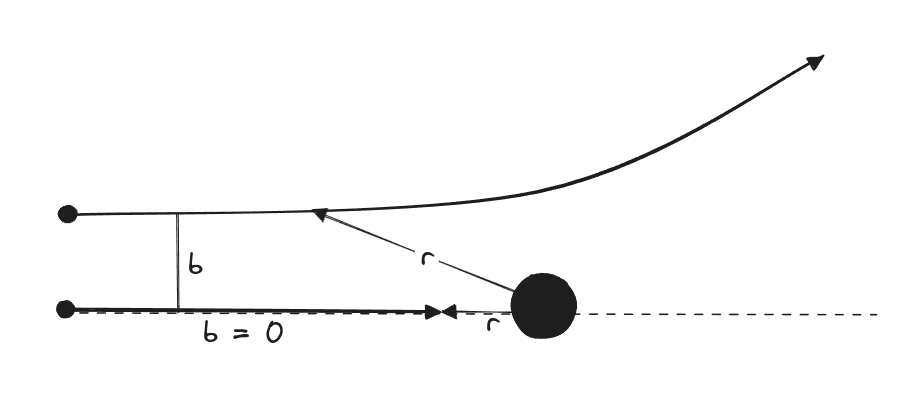
\includegraphics[scale=0.4]{ch3-48.png}
    \end{center}
    Let us consider the moment when the alpha particles are closest to the
    nuclear center. 
    Then at this moment, the alpha particle where $b \neq 0$ has a
    kinetic energy $K$ and a potential energy of $U = 2Zke^2/r_b$ hence
    \begin{align*}
        E = \frac{2Zke^2}{r_b} + K
    \end{align*}
    So for this alpha particle, the closest distance to the nucleus will be at
    \begin{align*}
        r_b = \frac{2Zke^2}{E - K}
    \end{align*}

    In the case where $b = 0$, the alpha particle will get close to the nucleus
    and for a moment this alpha particle will come to rest where $K = 0$.
    This is the moment where the alpha particle will be the closest to the 
    nucleus hence at this moment we will have that
    \begin{align*}
        E = \frac{2Zke^2}{r_0}
    \end{align*}
    Thus 
    \begin{align*}
        r_0 = \frac{2Zke^2}{E}
    \end{align*}
    Finally, we see that $r_0 < r_b$ since $K \geq 0$ and therefore the 
    the alpha particle that approaches the nucleus head-on gets closer to the
    nucleus than any other.
\end{proof}

\end{document}
